\chapter{Introduction}
\label{cha:introduction}

\section{Overview and aims}

\section{Dynamics of the polar stratosphere}

\subsection{Zonal mean flow}
\subsection{Planetary waves in the stratosphere}
\subsection{Stratospheric sudden warmings}


\section{Stratosphere-troposphere coupling}

\subsection{Influence of the troposphere on the stratosphere}
\subsection{Influence of the stratosphere on the troposphere}
\subsubsection{Observational evidence}
\subsubsection{Modelling evidence}
\subsubsection{Mechanisms}

% Look at Song and Robinson 2004 for basis of mechanisms review


\section{Thesis plan}

\begin{figure}
 \centering
 \noindent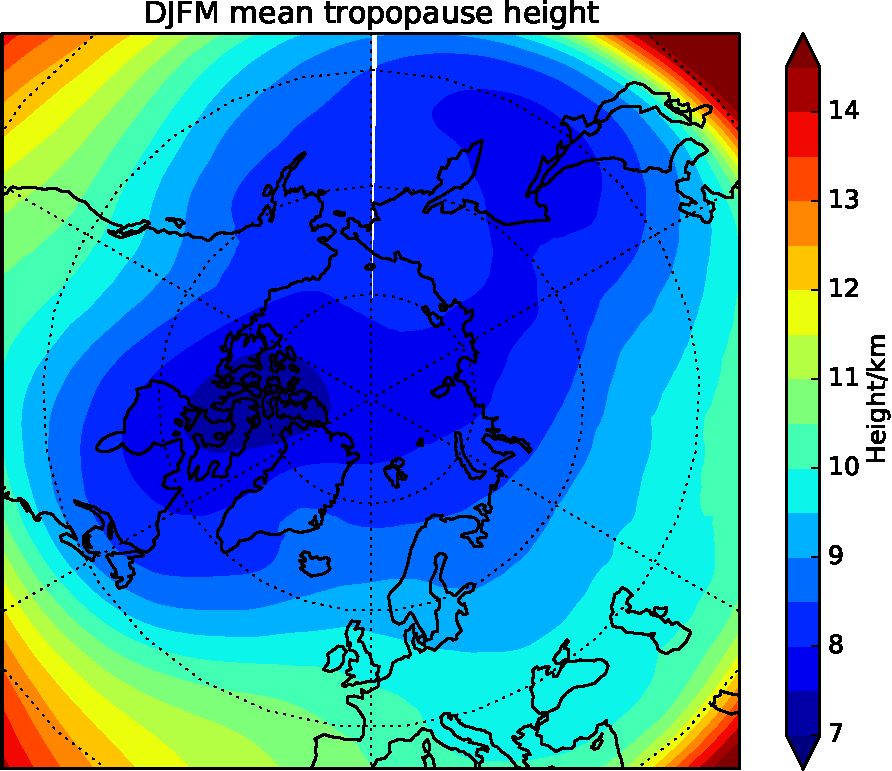
\includegraphics[width=0.5\textwidth]{figures/chapter-intro/mean_tropopause_height.pdf}
 \caption[]{ }
 \label{fig:cmip5_mslp_diff}
\end{figure}



%%% Local Variables:
%%% mode: latex
%%% TeX-master: "thesis"
%%% End:
